% musicar 450M base (464M): the pretrained multi-instrument model, without captions. Same look as the poster
% architecture.tex (its preamble is figstyle.tex): teal = model structure, grey boxes = linear layers and embedding
% tables, dashed frame = a module drawn open in place, dotted frame or box = a zoom into the dotted part. Sections are
% numbered in reading order.
% Sources: shapes from musicar/model/gpt.py; model_args, parameter counts (464,237,120: trunk 445,976,192, heads
% 16,275,456, embeddings 1,985,472) and the training config from checkpoints/long_450m_final/model_bf16.pt; recipe from
% config/pretrain/long_450m.py; final eval line from checkpoints/long_450m_final/train_tail.log (agents.md 2026-10-05);
% curve from curves/base_450m.dat (python docs/figures/curves_data.py parses the run log).
% Build (in docs/figures): pdflatex base_450m.tex
% PNG / SVG: pdftoppm -r 200 -png -singlefile base_450m.pdf base_450m ; pdftocairo -svg base_450m.pdf base_450m.svg
\documentclass[border=8pt]{standalone}
% Shared preamble of the per-model diagrams (base_450m.tex, base_107m_band.tex, base_107m_piano.tex,
% base_models.tex): packages, colours, TikZ styles and macros copied unchanged from architecture.tex, so they look
% the same. Use after \documentclass[border=8pt]{standalone}; keep in sync when the poster's style changes.

\usepackage[T1]{fontenc}
\usepackage[scaled=0.92]{helvet}
\renewcommand{\familydefault}{\sfdefault}
\usepackage{inconsolata}
\usepackage{amsmath}
\usepackage[italic]{mathastext}     % maths letters and digits in Helvetica, like the text
\usepackage[table]{xcolor}
\usepackage{array}
\usepackage{tabularx}
\usepackage{pgfplots}
\pgfplotsset{compat=1.18}
\usepackage{tikz}
\usetikzlibrary{arrows.meta,calc,decorations.pathreplacing,backgrounds}
\usepackage[hidelinks]{hyperref}
\hyphenpenalty=10000
\exhyphenpenalty=10000

\definecolor{tealT}{HTML}{3B7D70}   % title, structure labels, section numbers, brace
\definecolor{tealF}{HTML}{C3E0D6}   % repeated block, table header
\definecolor{tealB}{HTML}{6FA696}
\definecolor{greyF}{HTML}{F2F2F2}   % containers, text panels
\definecolor{greyB}{HTML}{8A8A8A}
\definecolor{rowG}{HTML}{F2F2F2}    % alternating table rows
\definecolor{pinkL}{HTML}{C2577A}   % captions: lines, labels
\definecolor{pinkF}{HTML}{F6CCD9}
\definecolor{boxG}{HTML}{D5D5D5}    % linear layers, embedding tables
\definecolor{altG}{HTML}{767676}    % curves: the alternative a choice was compared with (teal = what the model uses)

\tikzset{
  box/.style={draw=black, fill=white, rounded corners=3pt, minimum height=5.6mm, inner sep=3pt, align=center,
              font=\footnotesize, line width=0.6pt},
  gbox/.style={box, fill=boxG},
  pbox/.style={box, fill=pinkF, draw=pinkL},
  sub/.style={draw=tealB, dashed, rounded corners=6pt, line width=0.9pt},
  sublab/.style={text=tealT, font=\footnotesize\bfseries},
  zoom/.style={draw=black, densely dotted, rounded corners=10pt, line width=1.5pt},
  zline/.style={densely dotted, line width=1.5pt},
  panel/.style={draw=greyB, fill=greyF, rounded corners=8pt, line width=1pt},
  ptitle/.style={font=\small\bfseries, anchor=south west, inner sep=2pt},
  arr/.style={-{Stealth[length=2.4mm]}, line width=0.9pt},
  parr/.style={arr, draw=pinkL},
  sum/.style={draw=black, fill=white, circle, inner sep=0pt, minimum size=4.6mm, line width=0.8pt},
  tok/.style={draw=black, fill=white, minimum width=2.9mm, minimum height=2.9mm, inner sep=0pt, line width=0.4pt},
  ptok/.style={tok, fill=pinkF, draw=pinkL},
  note/.style={font=\scriptsize, text=black!85, align=left},
  ptext/.style={font=\footnotesize, text=black!90, align=left, inner sep=8pt},
  head/.style={box, minimum width=9mm, minimum height=7.5mm, inner sep=1pt, densely dotted, line width=1.1pt},
}
\newcommand{\rcite}[1]{{\scriptsize[#1]}}
\newcommand{\capt}[1]{\textcolor{pinkL}{``#1''}}
\newcommand{\badge}[1]{\tikz[baseline=(b.base)]\node[circle, fill=tealT, text=white, inner sep=0pt, minimum size=4.4mm,
  font=\scriptsize\bfseries] (b) {#1};}
\newcommand{\sect}[2]{\badge{#1}\hspace{4pt}#2}

\pgfplotsset{cplot/.style={scale only axis, width=5.3cm, height=3.3cm, axis lines*=left, axis line style={black!55},
  tick style={black!55}, grid=major, grid style={black!10}, tick label style={font=\scriptsize}, label style={font=\scriptsize},
  every axis plot/.append style={line join=round}, clip=false, xlabel shift=-2pt, ylabel shift=-3pt,
  scaled ticks=false, tick label style={/pgf/number format/fixed}}}


\tikzset{
  rollnote/.style={draw=black, fill=white, line width=0.5pt, rounded corners=1pt},
  dim/.style={{Stealth[length=1.3mm]}-{Stealth[length=1.3mm]}, line width=0.45pt},
}

\begin{document}%
%% ================= 1: one note = one compound token =================
\newsavebox{\rollBox}%
\sbox{\rollBox}{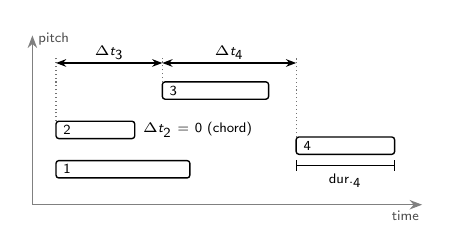
\begin{tikzpicture}
  \draw[black!50, line width=0.5pt, -{Stealth[length=1.6mm]}] (0, 0) -- (4.95, 0);
  \node[font=\tiny, text=black!70, anchor=north east, inner sep=1pt] at (4.95, -0.04) {time};
  \draw[black!50, line width=0.5pt, -{Stealth[length=1.6mm]}] (0, 0) -- (0, 2.15);
  \node[font=\tiny, text=black!70, anchor=west, inner sep=2pt] at (0, 2.1) {pitch};
  % notes 1 + 2: a chord (same onset), then 3, then 4
  \foreach \a/\b/\y/\n in {0.3/2.0/0.45/1, 0.3/1.3/0.95/2, 1.65/3.0/1.45/3, 3.35/4.6/0.75/4} {
    \draw[rollnote] (\a, \y-0.11) rectangle (\b, \y+0.11);
    \node[font=\tiny, inner sep=0pt] at (\a+0.14, \y) {\n};
  }
  \draw[densely dotted, black!55, line width=0.4pt] (0.3, 1.06) -- (0.3, 1.86);
  \draw[densely dotted, black!55, line width=0.4pt] (1.65, 1.56) -- (1.65, 1.86);
  \draw[densely dotted, black!55, line width=0.4pt] (3.35, 0.86) -- (3.35, 1.86);
  \draw[dim] (0.3, 1.8) -- (1.65, 1.8) node[midway, above, font=\tiny, inner sep=1pt] {$\Delta t_3$};
  \draw[dim] (1.65, 1.8) -- (3.35, 1.8) node[midway, above, font=\tiny, inner sep=1pt] {$\Delta t_4$};
  \node[font=\tiny, anchor=west, inner sep=1pt] at (1.36, 0.95) {$\Delta t_2 = 0$ (chord)};
  \draw[line width=0.45pt] (3.35, 0.5) -- (4.6, 0.5);
  \draw[line width=0.45pt] (3.35, 0.43) -- (3.35, 0.57);
  \draw[line width=0.45pt] (4.6, 0.43) -- (4.6, 0.57);
  \node[font=\tiny, anchor=north, inner sep=1.5pt] at (3.975, 0.45) {dur.$_4$};
\end{tikzpicture}}%

\newsavebox{\noteTab}%
\sbox{\noteTab}{\scriptsize\renewcommand{\arraystretch}{1.18}%
\begin{tabular}{@{\hspace{3pt}}>{\bfseries}l@{\hspace{5pt}}r@{\hspace{6pt}}>{\raggedright\arraybackslash}p{3.05cm}@{\hspace{3pt}}}
\rowcolor{tealF}\textcolor{tealT}{field} & \textcolor{tealT}{\textbf{values}} & \textcolor{tealT}{\textbf{meaning}}\\
\rowcolor{white}$\boldsymbol{\Delta t}$ & 512 & time since the previous note started (20 ms steps)\\
instr. & 129 & General MIDI program 0--127 or drums\\
\rowcolor{white}pitch & 130 & MIDI pitch 0--127 + start / end of a piece (BOS / EOS)\\
dur. & 512 & note length (20 ms steps)\\
\rowcolor{white}vel. & 32 & velocity: how hard the note is played\\
\end{tabular}}%

%% ================= 2: input embedding zoom =================
\newsavebox{\embZoom}%
\sbox{\embZoom}{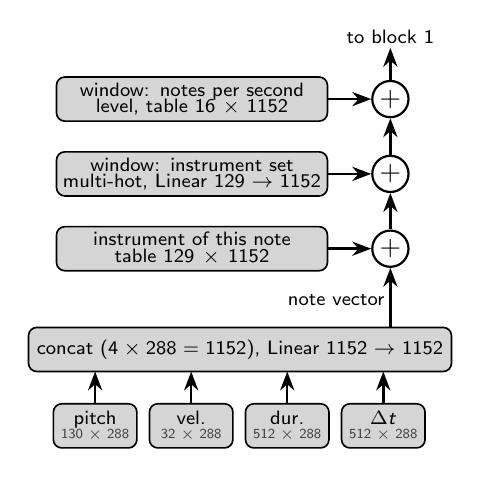
\begin{tikzpicture}
  \foreach \n/\v [count=\i] in {pitch/130, vel./32, dur./512, $\Delta t$/512} {
    \node[gbox, minimum width=10.6mm, font=\scriptsize, inner sep=2pt] (e\i) at (1.22*\i-0.62, 0) {\n\\[-3pt] {\tiny\textcolor{black!75}{$\v\times288$}}};
    \draw[arr] (e\i.north) -- (1.22*\i-0.62, 0.69);
  }
  \node[gbox, minimum width=47mm, font=\scriptsize] (cat) at (2.44, 0.97) {concat ($4\times288 = 1152$), Linear $1152\to1152$};
  \def\sx{4.35}
  \node[sum] (s1) at (\sx, 2.25) {$+$};
  \node[sum] (s2) at (\sx, 3.2) {$+$};
  \node[sum] (s3) at (\sx, 4.15) {$+$};
  \draw[arr] (\sx, 1.25) -- (s1);
  \node[font=\scriptsize, anchor=east, inner sep=2pt] at (\sx, 1.6) {note vector};
  \draw[arr] (s1) -- (s2);
  \draw[arr] (s2) -- (s3);
  \draw[arr] (s3) -- (\sx, 4.8) node[above, font=\scriptsize, inner sep=1pt] {to block 1};
  \node[gbox, font=\scriptsize, text width=33mm, inner sep=2pt] (b1) at (1.83, 2.25) {instrument of this note\\[-2pt] table $129\times1152$};
  \node[gbox, font=\scriptsize, text width=33mm, inner sep=2pt] (b2) at (1.83, 3.2) {window: instrument set\\[-2pt] multi-hot, Linear $129\to1152$};
  \node[gbox, font=\scriptsize, text width=33mm, inner sep=2pt] (b3) at (1.83, 4.15) {window: notes per second\\[-2pt] level, table $16\times1152$};
  \draw[arr] (b1) -- (s1);
  \draw[arr] (b2) -- (s2);
  \draw[arr] (b3) -- (s3);
\end{tikzpicture}}%

%% ================= 5: generation =================
\newsavebox{\genBox}%
\sbox{\genBox}{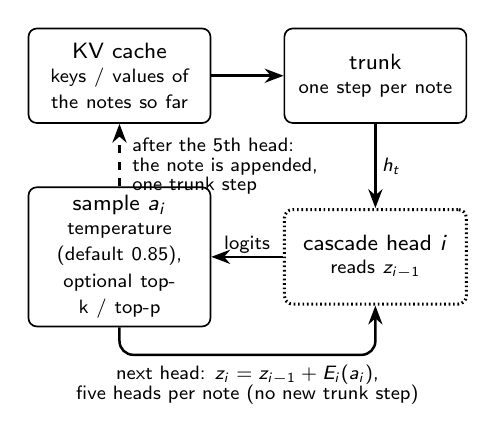
\begin{tikzpicture}
  \node[box, text width=21mm, minimum height=12mm] (kv) at (0, 2.3) {KV cache\\[-1pt] {\scriptsize keys / values of the notes so far}};
  \node[box, text width=21mm, minimum height=12mm] (tr) at (3.25, 2.3) {trunk\\[-1pt] {\scriptsize one step per note}};
  \node[box, text width=21mm, minimum height=12mm, densely dotted, line width=1.1pt] (hd) at (3.25, 0) {cascade head $i$\\[-1pt] {\scriptsize reads $z_{i-1}$}};
  \node[box, text width=21mm, minimum height=12mm] (sm) at (0, 0) {sample $a_i$\\[-1pt] {\scriptsize temperature (default 0.85), optional top-k / top-p}};
  \draw[arr] (kv) -- (tr);
  \draw[arr] (tr) -- node[right, font=\scriptsize, inner sep=2pt] {$h_t$} (hd);
  \draw[arr] (hd) -- node[above, font=\scriptsize, inner sep=1pt] {logits} (sm);
  \draw[arr, rounded corners=5pt] (sm.south) -- ++(0, -0.35) -| node[pos=0.25, below, font=\scriptsize, align=center] {next head: $z_i = z_{i-1} + E_i(a_i)$,\\[-1pt] five heads per note (no new trunk step)} (hd.south);
  \draw[arr, dashed] (sm.north) -- (kv.south);
  \node[font=\scriptsize, anchor=west, align=left, inner sep=1pt] at (0.12, 1.15) {after the 5th head:\\[-1pt] the note is appended,\\[-1pt] one trunk step};
\end{tikzpicture}}%


\newsavebox{\optBox}%
\sbox{\optBox}{\scriptsize\renewcommand{\arraystretch}{1.1}%
\newcommand{\opt}[2]{\hangindent=1.2em\hangafter=1 \texttt{#1}\ \ #2\\}%
\begin{tabular}{@{}>{\raggedright\arraybackslash}p{5.6cm}@{}}
{\footnotesize\textbf{generate.py options}}\\[1pt]
\opt{-{}-prompt f.mid}{continue a MIDI file}
\opt{-{}-sample-instruments}{sample each note's instrument (else all piano)}
\opt{-{}-instruments 0,33,128}{with it: the allowed programs (128~=~drums)}
\opt{-{}-cond-instruments, -{}-cond-density}{the window conditions: a program list / notes per second, prompt, or none}
\opt{-{}-temperature, -{}-top-p}{all heads (T 0.85 by default)}
\end{tabular}}%

%% ================= 6: pretraining =================
\newsavebox{\curveBase}%
\sbox{\curveBase}{\begin{tikzpicture}
\begin{axis}[cplot, xmin=0, xmax=8.3, ymin=1.6, ymax=2.9, xtick={0,2,4,6,8}, ytick={1.6,1.8,2.0,2.2,2.4,2.6,2.8},
    xlabel={notes seen (billions)}, ylabel={val CE (nats / note)}]
  \fill[tealF!55] (axis cs:6.636, 1.6) rectangle (axis cs:8.3, 2.9);
  \node[anchor=north, font=\scriptsize, text=black!75, align=center] at (axis cs:7.47, 2.88) {WSD\\cooldown};
  \addplot[tealT, line width=1.6pt] table[x=notes, y=ce] {curves/base_450m.dat};
  \fill[tealT] (axis cs:8.2956, 1.679) circle (2.2pt);
  \node[anchor=west, font=\scriptsize, text=black!85] at (axis cs:8.4, 1.679) {1.679};
  \node[anchor=south west, font=\scriptsize, text=black!85] at (axis cs:0.25, 2.807) {2.807 at 0.13B};
\end{axis}
\end{tikzpicture}}%

\newsavebox{\trainBox}%
\sbox{\trainBox}{\footnotesize\renewcommand{\arraystretch}{1.22}%
\begin{tabularx}{14.55cm}{@{\hspace{7pt}}>{\raggedright}p{2.3cm}>{\raggedright\arraybackslash}X@{\hspace{7pt}}}
\rowcolor{tealF}\textcolor{tealT}{\textbf{Setting}} & \textcolor{tealT}{\textbf{Base pretraining (done)}}\\
\rowcolor{white}Data & GigaMIDI 0.4, Aria-MIDI 0.3, Discover MIDI 0.3 (sampling weights); no audio-derived songs\\
Notes seen & 8.3B ($\approx$1.8 epochs on average; Aria-MIDI $\approx$4.5)\\
\rowcolor{white}Steps, batch & 126,582 steps $\times$ 65,536 notes (32 windows of 2,048 notes)\\
Optimizer & Muon (Moonlight scaling) for the weight matrices of the blocks, AdamW for the rest; one LR $10^{-3}$, weight decay 0.1\\
\rowcolor{white}Schedule & WSD: 1,000 warmup steps, constant LR, then ${1-\sqrt{\cdot}}$ decay to 0 over the last 20\%\\
Loss & sum of the five cross-entropies, teacher forcing; no dropout, no label smoothing\\
\rowcolor{white}Augmentation & random transposition by up to $\pm$5 semitones (drums unchanged)\\
Conditions & instrument set and density replaced by ``none'' in 15\% of the windows\\
\rowcolor{white}Precision & bf16 with fp8 matmuls, torch.compile; the checkpoint holds bf16 weights\\
Hardware & one rented RTX 5090, $\approx$41 h\\
\rowcolor{white}Result & clean GigaMIDI validation \textbf{1.679} nats / note = $\Delta t$ 0.170 + pitch 0.367 + dur.\ 0.644 + vel.\ 0.497
  (the instrument head, 0.117, apart); 1.681 with both conditions ``none''\\
\end{tabularx}}%

\begin{tikzpicture}

%% ================= title =================
\node[font=\fontsize{20}{22}\selectfont\bfseries, text=tealT] at (-0.2, 19.95) {musicar 450M base (464M)};
\node[font=\footnotesize, text=black!85] at (-0.2, 19.3) {Pretrained multi-instrument MIDI model without text captions: 464.24M parameters (trunk 445.98M,
  cascade heads 16.28M, embeddings 1.99M), trained on 8.3B notes.};
\node[font=\scriptsize, text=black!75] at (-0.2, 18.75) {How to read: numbers give the reading order; teal = the model's structure; grey boxes = linear layers
  and embedding tables; dashed frame = a module drawn open in place; dotted frame or box = a zoom into the dotted part.};

%% ================= 3: main column =================
\node[ptitle] at (-4.3, 17.35) {\sect{3}{Music model}};
\begin{scope}[on background layer]
  \fill[tealF, draw=tealB, rounded corners=12pt, line width=0.8pt] (-3.6, 3.3) rectangle (3.6, 11.6);
\end{scope}

% input
\node[box] (inp) at (0, -0.65) {Note tokens {\scriptsize (one position = one note: $\Delta t$, instr., pitch, dur., vel.)}};
\node[font=\footnotesize, text=black!85] at (0, -1.35) {a window of up to 2,048 notes ($\approx$1--4 min of music)};
\draw[arr] (inp) -- (0, 0.67);

% embedding + conditions
\node[gbox, densely dotted, line width=1.1pt] (emb) at (0, 0.95) {Note embedding {\scriptsize ($4\times288$, concat, Linear)}};
\node[sum] (s0) at (0, 1.85) {$+$};
\node[gbox, densely dotted, line width=1.1pt, font=\scriptsize] (cond) at (-2.5, 1.9) {Instrument (per note)\\[-2pt] + instr. set, density\\[-2pt] (per window)};
\draw[arr] (emb) -- (s0);
\draw[arr] (cond.east |- s0) -- (s0);
\node[tok] at (1.05, 1.85) {};
\node[note, anchor=west] at (1.25, 1.85) {note vector (1152)};

% the sequence: one vector per note
\foreach \k in {-8,...,8} { \node[tok] at (0.32*\k, 2.75) {}; }
\node[font=\scriptsize] at (2.95, 2.75) {$\cdots$};
\node[text=black!75, font=\tiny, anchor=south] at (-2.56, 2.9) {note 1};
\node[text=black!75, font=\tiny, anchor=south] at (2.95, 2.9) {2,048};
\draw[arr] (s0) -- (0, 2.6);

% transformer block
\node[box, minimum width=26mm] (ln1) at (0, 4.3) {RMSNorm 1};
\node[box, minimum width=36mm, minimum height=8mm] (att) at (0, 5.75) {Causal self-attention\\[-2pt] {\scriptsize 18 heads $\times$ 64, full attention}\\[-3pt]
  {\scriptsize Q, K, V each $1152\to18\times64$}\\[-3pt] {\scriptsize (one fused Linear $1152\to3456$)}\\[-3pt] {\scriptsize QK-norm, RoPE; output $1152\to1152$}};
\node[sum] (a1) at (0, 7.45) {$+$};
\node[box, minimum width=26mm] (ln2) at (0, 8.6) {RMSNorm 2};
\node[box, minimum width=36mm, minimum height=8mm] (ffn) at (0, 9.7) {SwiGLU feed-forward\\[-2pt] {\scriptsize $1152\to3072$ (gate and up) $\to1152$}};
\node[sum] (a2) at (0, 11.05) {$+$};
\draw[sub] (-2.3, 3.75) rectangle (2.3, 6.8);
\node[sublab, anchor=south west] at (-2.3, 6.8) {Attn sublayer};
\draw[sub] (-2.3, 8.1) rectangle (2.3, 10.4);
\node[sublab, anchor=south west] at (-2.3, 10.4) {FFN sublayer};
\draw[arr] (0, 2.9) -- (ln1);
\draw[arr] (ln1) -- (att);
\draw[arr] (att) -- (a1);
\draw[arr] (a1) -- (ln2);
\draw[arr] (ln2) -- (ffn);
\draw[arr] (ffn) -- (a2);
\draw[arr, rounded corners=4pt] (0, 3.55) -- (3.1, 3.55) |- (a1.east);
\draw[arr, rounded corners=4pt] (0, 7.85) -- (3.1, 7.85) |- (a2.east);
\fill (0, 3.55) circle (1.4pt);
\fill (0, 7.85) circle (1.4pt);

% repeat brace
\draw[decorate, decoration={brace, amplitude=7pt}, line width=1.2pt, draw=black] (-4.45, 3.3) -- (-4.45, 11.6);
\node[font=\fontsize{15}{17}\selectfont\bfseries, text=tealT, anchor=east] at (-4.75, 7.45) {28 $\times$};
\node[font=\scriptsize, text=tealT, anchor=north east] at (-4.75, 7.0) {445.98M};
\node[sublab, anchor=north west] at (-3.45, 11.45) {width 1152};

% final norm + cascade heads: a running state z (z_0 = h_t) read by each head, plus the embedding of each decided value
\node[box, minimum width=34mm] (lnf) at (0, 12.15) {Final RMSNorm};
\draw[arr] (a2) -- (lnf);
\draw[sub] (-4.05, 12.6) rectangle (4.05, 15.55);
\node[sublab, anchor=south east] at (4.0, 12.63) {Cascade heads {\scriptsize\mdseries (16.28M)}};
\def\ry{13.25}
\foreach \x/\n/\v [count=\i] in {-3.1/$\Delta t$/512, -1.55/instr./129, 0/pitch/130, 1.55/dur./512, 3.1/vel./32} {
  \node[head] (h\i) at (\x, 13.95) {\n\\[-3pt] {\tiny $V{=}\v$}};
  \node[tok, minimum width=5mm, minimum height=4mm, font=\scriptsize] (t\i) at (\x, 14.8) {$a_{\i}$};
  \draw[arr] (h\i) -- (t\i);
}
\foreach \x [count=\i] in {-3.1, -1.55, 0, 1.55} {
  \node[gbox, minimum width=4mm, minimum height=5.6mm, inner sep=1pt, font=\scriptsize] (e\i) at (\x+0.78, 13.95) {$E_{\i}$};
  \node[sum, minimum size=4mm] (c\i) at (\x+0.78, \ry) {$+$};
  \draw[arr, rounded corners=3pt] (t\i.east) -| (e\i.north);
  \draw[arr] (e\i) -- (c\i);
}
% the state rail, entered from the side of the final norm
\draw[line width=0.9pt, rounded corners=4pt] (lnf.west) -- (-3.85, 12.15) -- (-3.85, \ry) -- (-3.1, \ry);
\node[font=\scriptsize, anchor=south, inner sep=1pt] at (-3.48, \ry) {$h_t$};
\draw[arr] (-3.1, \ry) -- (c1.west);
\foreach \a/\b in {c1/c2, c2/c3, c3/c4} { \draw[arr] (\a.east) -- (\b.west); }
\draw[line width=0.9pt] (c4.east) -- (3.1, \ry);
\foreach \x [count=\i] in {-3.1, -1.55, 0, 1.55, 3.1} {
  \draw[arr] (\x, \ry) -- (h\i.south);
  \ifnum\i<5 \fill (\x, \ry) circle (1.4pt); \fi
}
% every head's value goes into its own field of the next note
\foreach \x/\n [count=\i] in {-3.1/$\Delta t$, -1.55/instr., 0/pitch, 1.55/dur., 3.1/vel.} {
  \node[draw=black, fill=white, minimum width=15.5mm, minimum height=5.5mm, inner sep=0pt, font=\footnotesize,
        line width=0.6pt] (o\i) at (\x, 16.6) {\n};
  \draw[arr] (t\i.north) -- (o\i.south);
}
\node[font=\footnotesize, anchor=south] at (0, 16.9) {Next note: one compound token};
% generation loop: the sampled note becomes the next input
\draw[arr, dashed, rounded corners=6pt] (o5.east) -- (4.85, 16.6) -- (4.85, -0.65) -- (inp.east);

%% ================= 1: one note (left, top) =================
\node[anchor=north west, text width=5.0cm, ptext, inner sep=8pt] (note) at (-12.0, 17.25) {%
\usebox{\rollBox}\\[3pt]
{\scriptsize Notes 1--4 become positions 1--4: one position per note, in onset order, each with all five
values:}\\[4pt]
\usebox{\noteTab}\\[5pt]
\textbf{Time is absolute:} no bars, beats or tempo tokens; $\Delta t$ and durations stop at 10.22 s. The notes of all
tracks are merged into one sequence; for drums the pitch is the drum sound.};
\begin{scope}[on background layer]
  \draw[panel] (note.south west) rectangle (note.north east);
\end{scope}
\node[ptitle] at (note.north west) {\sect{1}{One note = one compound token}};

%% ================= 2: input embedding zoom (left, bottom) =================
\node[anchor=north west, text width=5.0cm, ptext, inner sep=8pt, fill=white] (embz) at ($(note.south west)+(0, -0.9)$) {%
\usebox{\embZoom}\\[4pt]
The instr.\ head predicts the next note's instrument (128 General MIDI programs + drums). The two \textbf{window
conditions} are added at every position, measured on the window's own notes (density: 15 levels + ``none''). In
training both are replaced by ``none'' in 15\% of the windows, so ``none'' (unconditional) stays usable; in generation
they come from the user or the prompt. The instrument table and both conditions start at zero.};
\node[ptitle] at (embz.north west) {\sect{2}{Input embedding {\mdseries\footnotesize (1.99M)}}};
\draw[zline] (embz.east |- cond) -- (cond.west);
\draw[zline] (embz.east |- emb) -- (emb.west);

%% ================= 4: cascade head zoom (right, top) =================
\draw[zoom] (5.4, 12.45) rectangle (11.6, 17.25);
\node[ptitle] at (5.4, 17.35) {\sect{4}{One cascade head {\mdseries\footnotesize (one per dotted box)}}};
\def\hx{8.3}
\node[box] (rz) at (\hx, 13.0) {$z_{i-1}$ {\scriptsize (1152)}};
\node[gbox, minimum width=40mm] (r1) at (\hx, 13.8) {LayerNorm, Linear $1152\to1152$};
\node[gbox, minimum width=40mm] (r2) at (\hx, 14.55) {GELU, Linear $1152\to1152$};
\node[sum] (rs) at (\hx, 15.3) {$+$};
\node[gbox, minimum width=40mm] (ro) at (\hx, 16.0) {LayerNorm, Linear $1152\to V$};
\draw[arr] (rz) -- (r1);
\draw[arr] (r1) -- (r2);
\draw[arr] (r2) -- (rs);
\draw[arr] (rs) -- (ro);
\draw[arr] (ro) -- (\hx, 16.57) node[above, font=\scriptsize, inner sep=1pt] {logits over the $V$ values};
\fill (\hx, 13.38) circle (1.4pt);
\draw[arr, rounded corners=4pt] (\hx, 13.38) -- (10.75, 13.38) |- (rs.east);
\node[anchor=north west, text width=6.2cm, font=\footnotesize, text=black!90, align=left, inner sep=0pt] (why) at (5.4, 12.2) {%
\textbf{Why a cascade.} One position predicts all five values of the next note. Head $i$ reads the running state\\[2pt]
\hspace*{0.5cm}$z_0 = h_t,\quad z_i = z_{i-1} + E_i(a_i)$,\\[2pt]
the trunk state $h_t$ plus the embeddings $E$ of the values already chosen
(tables $512$, $129$, $130$, $512\times1152$; the last head needs none). So the note's probability follows the
chain rule:\\[2pt]
\hspace*{0.5cm}$p(\Delta t)\,p(\text{instr.}\mid\Delta t)\,p(\text{pitch}\mid\Delta t,\text{instr.})\cdots$\\[3pt]
Each head has its own weights. $a_i$ is the true value in training (teacher forcing) and the sampled value in
generation. Loss: the sum of the five cross-entropies. In a 42M test, the same heads without the chain were $+0.34$ nats / note worse.};

%% ================= 5: generation (right, bottom) =================
\path let \p1 = (why.south) in coordinate (G) at (5.4, \y1 - 0.85cm);
\node[anchor=north west, inner sep=9pt] (gend) at (G) {\usebox{\genBox}};
\node[anchor=north west, text width=5.6cm, ptext, inner sep=0pt] (gent) at ($(gend.south west)+(0.3, 0)$) {%
Start from BOS or from a MIDI prompt; EOS ends the piece. Past 2,048 notes the window slides by a quarter.\\[5pt]
\usebox{\optBox}};
\node[ptitle] at (gend.north west) {\sect{5}{Generation}};

%% ================= the three columns end at the same height =================
\path let \p1 = (embz.south), \p2 = (gent.south), \n1 = {min(\y1, \y2 - 9pt, -1.75cm)} in coordinate (Bot) at (0, \n1);
\begin{scope}[on background layer]
  \path let \p1 = (Bot) in [fill=greyF, draw=greyB, rounded corners=16pt, line width=1pt] (-4.3, \y1) rectangle (4.3, 16.05);
  \path let \p1 = (Bot) in [panel] (gend.north west) rectangle (11.6, \y1);
\end{scope}
\path let \p1 = (Bot) in [zoom] (embz.north west) rectangle (embz.east |- 0, \y1);

%% ================= 6: pretraining (bottom strip) =================
\path let \p1 = (Bot) in coordinate (C) at (-12.0, \y1 - 1.0cm);
\node[anchor=north west, text width=7.6cm, font=\scriptsize, text=black!85, align=left, inner sep=10pt] (cv) at (C) {%
  {\footnotesize\bfseries Clean GigaMIDI validation (8.3B notes)}\\[3pt]
  \usebox{\curveBase}\\[2pt]
  Every 2,000 steps (65,536 notes per step): the sum of the $\Delta t$, pitch, duration and velocity cross-entropies on
  GigaMIDI validation files whose notes do not occur in its training split. Constant LR, then the ${1-\sqrt{\cdot}}$~cooldown in the
  last 20\%. One run.};
\node[anchor=north west, inner sep=0pt] (tab) at ($(cv.north east)+(0.35, -0.35)$) {\usebox{\trainBox}};
\path let \p1 = (cv.south), \p2 = (tab.south), \n1 = {min(\y1, \y2 - 10pt)} in coordinate (Cs) at (11.6, \n1);
\begin{scope}[on background layer]
  \draw[panel] (C) rectangle (Cs);
\end{scope}
\node[ptitle] at (C) {\sect{6}{Pretraining}};

\end{tikzpicture}
\end{document}
